\documentclass[a4paper,11pt]{article}
\usepackage[a4paper, margin=3cm]{geometry}
\usepackage[spanish]{babel}%Para el español
\usepackage[utf8]{inputenc}%para los acentos	
\usepackage{amsmath,amssymb,amsfonts,amsthm}
\usepackage{graphicx}
\usepackage{lmodern}
\usepackage[T1]{fontenc}
%----------------------------
\usepackage{xcolor}
\usepackage{listings}

\lstset{
	language=Octave,
	basicstyle=\small\ttfamily,
    keywordstyle=\bfseries\color[rgb]{0,0,1},
    commentstyle=\color[rgb]{0.13,0.54,0.13},
    %0.133333 0.545098 0.133333
    stringstyle=\ttfamily\color{red!50!brown},
	literate=%
	{á}{{\'{a}}}1
    {é}{{\'{e}}}1
    {í}{{\'{i}}}1
    {ó}{{\'{o}}}1
    {ú}{{\'{u}}}1
    {ñ}{{\~{n}}}1
    {<}{{$<$}}1
    {>}{{$>$}}1
    {_}{{\_}}1,    
    frame=single,
    %inputencoding=utf8,
	%extendedchars=false,
	%upquote=true,
    breaklines=true,
    postbreak=\raisebox{0ex}[0ex][0ex]{\ensuremath{\color{red}\hookrightarrow\space}},
}
\usepackage{textcomp}%me dejó usar el simbolo de grados (°)
\usepackage{gensymb}%me dejó usar \degree para las fórmulas
\usepackage{subfig}%me dejó modificar la distancia de las epigrafes.
\usepackage{float}%me dejó fijar la posicion de las impagenes
\usepackage{footnote}
\makesavenoteenv{tabular}
\makesavenoteenv{table}
\usepackage[font=scriptsize,labelfont=bf]{caption}
%\usepackage[spanish,activeacute]{babel}
\graphicspath{{Imagenes/}}
\captionsetup{belowskip=12pt,aboveskip=4pt}


\title{Sistemas de Control I \\ Monografía: 
\\Implementación de sistema de control automático para regulación de la intensidad lumínica\\}

\author{\\Alumno:Morales Esteban Andrés Matrícula:35104714\\
	  Docente:Ing. Reyes Reinaldo.}
\begin{document}
% genera el titulo
\maketitle
\newpage
% inserta la table de contenidos
\tableofcontents
\newpage
\section{Descripción del problema}
En el presente trabajo se describirá el proceso de desarrollo de un sistema de control automático para regular la intensidad lumínica en una habitáculo.Siendo una posible aplicación práctica la industria de la fotografía por ejemplo sobre-exposiciones o captura de procesos largos en timelapse.Por ejemplo algunos fenómenos biológicos o químicos requieren que se tomen muchas tomas pero sería optimo conservar el nivel de iluminación para evitar el post-procesamiento de las imágenes.
En un enfoque inicial se plantea un sistema de lazo abierto conformado por 4 componentes principales
\begin{itemize}
	\item Potenciómetro (Resistencia Variable)
	\item Arduino UNO
	\item Circuito Dimmer (Corte Alterna)
	\item Lámpara de filamento incandescente
\end{itemize}

\begin{figure}[H] % Example image
	\center{\includegraphics[width=0.9\linewidth]{remake/esquema_ilustrativo.png}}
	\caption{Esquema ilustrativo.}
	\label{fig:esquema_ilustra}
\end{figure} 

En una instancia posterior se incorporará al diseño original un sensor LDR (Light Diode Resistense) de luminosidad para medir el nivel de iluminación proporcionado por la lampara y de esta manera ofrecer un punto de retroalimentación al sistema inicial. 
\\
Se debe mencionar que el sistema deberá ser capaz de soportar perturbaciones exteriores, como ser la apertura de ventanas o alguna sombra que pueda producirse por distintas causas, que pueden provenir por el paso de una persona, o de nubes.

%TODO revisar valores. Me parece que la determinación del rango de control se realiza en la etapa de analisi temporal en lazo abierto
La entrada del sistema sera 0V a 10V, que se relacionaran con la salida de forma lineal. El rango de salida del sistema sera de 0lm a 1000lm. Se seleccionará una entrada deseada, por ej 8V al que le corresponde una salida de 800lm, y el sistema deberá ser capaz de mantener la salida correspondiente, a pesar de las perturbaciones consideradas.

\subsection{Potenciómetro}
Una resistencia variable utilizada a modo de divisor de tensión permitirá fijar un nivel de control.
\begin{figure}[H] % Example image
	\center{\includegraphics[width=0.3\linewidth]{remake/pote_divisor.png}}
	\caption{Esquema circuito potenciometro.}
	\label{fig:potenciometro}
\end{figure} 

\subsection{Arduino Uno}
Una placa de prototipado digital que incluye un microcontrolador de la marca Atmel ATmega328 será utilizada para medir la señal de ajuste del potenciómetro y permitirá generar las señales de control para el circuito de dimmerización.\\
El microcontrolador funciona por defecto a una velocidad de reloj de 16Mhz lo que se traduce en un tiempo de ejecución de instrucción de aproximadamente 25 ns.\\
Utilizando la librería en C oficial de arduino se consiguen lecturas del ADC cada 100 us y lecturas digitales con una demora de 5 us en promedio por lo que deberán contemplarse dichas demoras en el análisis de las respuestas temporales de cada bloque si fuesen significativas.\\
Debido a que el rango de tensión especificado como señal de referencia va de 0v a 10v será necesario incluir un divisor resistivo ya que los pines analógicos de esta placa soportan un máximo de 3.3v.
Se calcula el divisor resistivo.

\begin{figure}[H] % Example image
	\center{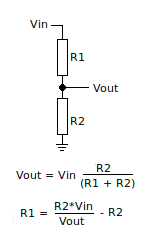
\includegraphics[width=0.2\linewidth]{divisor_general}}
	\caption{Esquemático genérico para el divisor.}
	\label{fig:divisor_general}
\end{figure} 

Si asumo un valor común en el orden de los $K\Omega$ para R2 puedo calcular R1.\\
Sea $R2=1K\Omega$, entonces:\\
$$R_1 = \frac{R_2\times V_in}{V_out} - R_2$$
$$R_1 = \frac{1K\Omega\times 10v}{3.3v} - 1K\Omega$$
$$R_1 \approx 2K\Omega$$

\subsection{Dimmer}
Circuito electrónico capaz de detectar cruzes por cero de una señal alterna para los que generará una señal de niveles digitales y corta duración preparada para ser medida.\\
Al mismo tiempo el circuito ofrece una etapa de recorte de la señal alterna de entrada mediante el empleo de un TRIAC.\\
A continuación se muestra un esquema ilustrativo del circuito a ser empleado.

\begin{figure}[H] % Example image
	\center{\includegraphics[width=0.8\linewidth]{remake/001__circuito_dimmer.jpg}}
	\caption{Esquema circuito dimmer.}
	\label{fig:circ_dimmer}
\end{figure} 
 
 El efecto de la polarización de la compuerta del TRIAC T1 produce una deformación o corte de la señal alterna original. Tal efecto puede observarse en la forma de onda percibida por la lámpara.
 
 \begin{figure}[H] % Example image
 	\center{\includegraphics[width=0.7\linewidth]{remake/003__gate_chopped.png}}
 	\caption{Principio de acción sobre la señal original.}
 	\label{fig:gate_chopped}
 \end{figure} 
 
\begin{figure}[H] % Example image
	\center{\includegraphics[width=0.7\linewidth]{remake/004__chopped_examples.png}}
	\caption{Ejemplos de deformación de la señal original.}
	\label{fig:chopped_examples}
\end{figure} 
 
 Como puede observarse de la acción de dimmerización la señal deformada cambia con los rertrasos introducidos por los componentes del circuito de dimmer.\\
 Los valores relevantes para este caso se toman en consideración:

\begin{itemize}
	\item Índice de conmutación TRIAC: 20 V/us
	\item Retardo por excitación de compuerta: 2 us
\end{itemize}

\textbf{PEOR ESCENARIO}
$$\widehat{V}_{RED} = 311v$$
$$t_{CONM} = \frac{1}{20}\frac{\mu s}{v}\times 311v$$
$$t_{CONM} = 15,55\mu s$$
$$t_{TOTAL} = 2\mu s + 15,55\mu s$$
$$t_{TOTAL} = 17,55\mu s$$

Sin embargo los efectos del cambio de $V_{RMS}$ aparente se verán completos una vez que termine el ciclo de alterna

$$F_{RED}=50Hz$$
$$T_{RED}=20\mu s$$

\subsection{Lámpara}
El diseño planteado sólo funcionará para lámaparas de filamento incandescente.
Según las especificaciones ofrecidas por OSRAM.
Para alcanzar el 90\% de la iluminación tabulada se requerirá un $t_{REAC}=250ms$
Si se supone la respuesta exponencial entonces 

\begin{align*}
& 90~\text{\small \% } \,\rule[2.5pt]{16pt}{0.5pt}\,
20~\text{\small ms}\\
& 63,2~\text{\small \%} \,\rule[2.5pt]{16pt}{0.5pt}\,
~\text{\small $\tau$}
\end{align*}
$$\tau = 175,5ms$$

Como observación general a pedido del evaluador se realizará un redondeo a 200ms para facilitar el cálculo a posterior.

\section{Planteo Inicial: Sistema sin Realimentación}
Teniendo en cuenta las consideraciones anteriores puede reducirse el planteo del sistema con el siguiente diagrama de bloques.

\begin{figure}[H] % Example image
	\center{\includegraphics[width=0.7\linewidth]{remake/005__sistema_sin_retro.png}}
	\caption{Planteo sistema sin realimentación.}
	\label{fig:sistema_sin_retro}
\end{figure} 
Para convertir el esquema en un sistema de control automático es necesario incorporar un componente de retroalimentación, un detector de errores o comparador.

\begin{figure}[H] % Example image
	\center{\includegraphics[width=0.7\linewidth]{remake/006__sistema_con_retro.png}}
	\caption{Planteo sistema con realimentación.}
	\label{fig:sistema_con_retro}
\end{figure} 
\subsection{Aclaración sobre el Bloque Actuador}
El bloque Actuador(Figura \ref{fig:sistema_sin_retro}) queda compuesto por:
\begin{itemize}
	\item Divisor resistivo para el pin analógico.
	\item Arduino.
	\item Circuito Cortador de señal Sinusoidal.
\end{itemize}
La señal de entrada a dicho bloque es la de referencia (0v-10v)DC y la de salida es el Voltaje RMS (Tensión Eficaz) con rango (0v - 220v)AC.\\
La razón de esconder la implementación en ese bloque a modo de caja negra es justamente evitar el análisis de las señales de intercambio entre el arduino y el circuito cortador.
Esto es porque la señal especificada como "Dimmer Signal In" (Figura \ref{fig:circ_dimmer}) ó "Gate Voltage" (Figura \ref{fig:gate_chopped}) NO es PWM.
El ancho del pulso siempre es el mismo (10 microsegundos según la implementación que investigué para el trabajo).\\
Lo que realmente varía es la distancia temporal t1 (Figura 5) desde el cruce por cero de la senoidal al inicio del pulso. Por eso existe la señal "Zero Crossing"(Figura \ref{fig:circ_dimmer}).
Mediante una calibración por software se convierte el valor leído por el ADC de la señal de referencia en el tiempo t1 correspondiente para conseguir el corte adecuado de la senoidal. 

\subsection{Sensor}
Como componente de lazo de feedback se eligió una Light Dependant Resistance (LDR) específicamente el modelo GL10516 de la serie 10 de sensores LDR de respuesta rápida configurada en una malla con divisor de tensión es posible conseguir un rango de voltajes adecuados.

El tiempo de respuesta de este dispositivo a cambios de luminosidad se especifica en la hoja de datos del componente provista por el fabricante y se establece en 30ms ya sea para el incremento de la resistencia o el decremento. Con esta información se calcula la constante de tiempo de respuesta como sigue:
\begin{align*}
& 100~\text{\small \% } \,\rule[2.5pt]{16pt}{0.5pt}\,
30~\text{\small ms}\\
& 63,2~\text{\small \%} \,\rule[2.5pt]{16pt}{0.5pt}\,
~\text{\small $\tau$}
\end{align*}
$$\tau = 19ms$$


\subsection{Funciones de Transferencia}
\subsubsection{ACTUADOR}
$$FT_{Actuador} =\frac{\frac{OUTPUT_{MAX}}{INPUT_{MAX}}}{1+\tau_{BLOQUE}\times s}$$
$$=\frac{\frac{220}{10}}{1+0,02 s}=\frac{22}{1+0,02 s}=\frac{22}{0,02(50+s)}$$
$$FT_{Actuador} = \frac{1100}{s+50}$$

\subsubsection{PLANTA}
$$FT_{Planta} =\frac{\frac{OUTPUT_{MAX}}{INPUT_{MAX}}}{1+\tau_{BLOQUE}\times s}$$
$$=\frac{\frac{1000}{220}}{1+0,2 s}=\frac{4,54}{1+0,02 s}=\frac{4,54}{0,2(5+s)}= \frac{22,7}{s+5}$$
$$FT_{Planta} = \frac{23}{s+5}$$

\subsubsection{SENSOR}
$$FT_{Sensor} =\frac{\frac{OUTPUT_{MAX}}{INPUT_{MAX}}}{1+\tau_{BLOQUE}\times s}$$
$$=\frac{\frac{10}{1000}}{1+0,05 s}=\frac{0,01}{1+0,05 s}=\frac{0,01}{0,05(20+s)}$$
$$FT_{Actuador} = \frac{0,53}{s+52.63}$$

\section{Función de Transferencia de Lazo Abierto}
Utilizando las funciones de transferencia previamente calculadas, se obtiene la función de transferencia de lazo abierto del sistema:
$$FT_{LA}=FT_{Actuador}  \times FT_{Planta} \times FT_{Sensor} $$
$$FT_{LA}=\frac{13409}{s^3 + 107.6 s^2 + 3145 s + 13160}$$
%\subsection{Analisis de la funcion de transferencia}
\begin{table}[h!]
\centering
\caption{Esta tabla muestra los datos obtenidos de la separación zpk.}
\begin{tabular}{|ccccc|}
\hline 
Ceros & Polos & Ganancia & Tipo \footnote{Debido a que el sistema no tiene polos al origen, el mismo es de tipo 0 (cero).} & Órden \tabularnewline
\hline 
\hline 
 No Tiene & -5 & 13409 & '0'(cero) & '3'(tres) \tabularnewline
 & -50 & & &\tabularnewline
 & -50.63 & & &\tabularnewline
\hline 
\end{tabular}
\end{table}

La función de transferencia en el modo \emph zpk es:
$$FT_{LA_{(ZPK)}}=\frac{13409}{(s + 5)(s + 50)(s + 50.63)}$$
A continuación se muestra el grafico de polos del sistema:
  \begin{figure}[H] % Example image
	\center{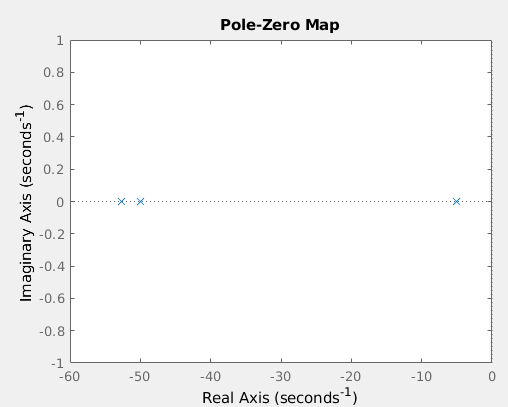
\includegraphics[width=0.7\linewidth]{FTlazoa_pzmap}}
	\caption{Gráfico de Polos y Ceros del Sistema.}
	\label{fig:cp1}
	\end{figure} 
Debido a que el sistema no posee polos en el origen, estamos en presencia de un sistema de tipo 0. El error de régimen permanente ante una señal de entrada escalón para estos casos se obtiene con la siguiente formula:
$$k_p=\lim\limits_{s\rightarrow 0}FT_{LA}(s) $$
$$k_p=\lim\limits_{s\rightarrow 0}\frac{13409}{(s + 5)(s + 50)(s + 50.63)} $$
$$k_p=\frac{13409}{5\times50\times50.63} $$
$$k_p= 1.02$$
$$e_{ss}=\frac{1}{k_p+1}=\frac{1}{2.02}=0,49\approx0.5 $$
Es decir, que el error en estado estable del sistema es del 50\%.
\section{Función de Transferencia de Lazo Directo}
La función de transferencia de lazo directo se calcula anulando el lazo de feedback osea solo se tendrá en cuenta los efectos del actuador y la planta en este caso:
$$FT_{LD}=\frac{25300}{s^2 + 55 s + 250}$$
$$FT_{LD_{(ZPK)}}=\frac{25300}{(s + 5)(s + 50)}$$
A continuación se observa la salida de la función de transferencia de lazo directo ante una entrada de 10V. Se puede ver que llega al valor máximo que se espera del sistema de 1000lm.

  \begin{figure}[H] % Example image
	\center{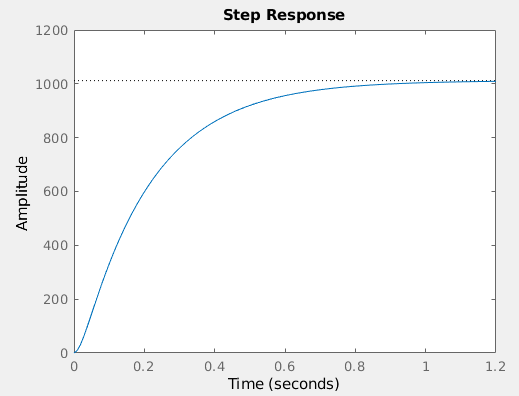
\includegraphics[width=0.7\linewidth]{FTlazod_step}}
	\caption{Gráfico de la respuesta del sistema a la entrada escalón de 10V.}
	\label{fig:resp_esc1}
	\end{figure} 

\section{Función de Transferencia de Lazo Cerrado}
La función de transferencia de lazo cerrado se consigue de la aritmética del diagrama de bloques y es la siguiente:
$$FT_{LC}=\frac{FT_{Actuador} \times FT_{Planta} }{1+FT_{Actuador}  \times FT_{Planta} \times FT_{Sensor}} $$
$$FT_{LC}=\frac{25300s+1332000}{s^3 + 107.6 s^2 + 3145 s + 26570}$$
Análisis de la función de transferencia:
\begin{table}[h!]
\centering
\caption{Esta tabla muestra los datos obtenidos de la separación zpk.}
\begin{tabular}{|ccccc|}
\hline 
 Ceros & Polos & Ganancia & Tipo \footnote{Debido a que el sistema no tiene polos al origen, el mismo es de tipo 0 (cero).} & Orden \tabularnewline
\hline 
\hline 
 -52.63 & -66.18 & $25300$ & '0'(cero) & '3'(tres) \tabularnewline
 & -26.03 & & &\tabularnewline
 & -15.42 & & &\tabularnewline
\hline 
\end{tabular}
\end{table}
La función de transferencia de lazo cerrado en el modo \emph zpk es:
$$FT_{LC_{(ZPK)}}=\frac{25300\times(s+52.63)}{(s + 66.18)(s + 26.03)(s + 15.42)}$$
La ecuación característica es:  
$$s^3 + 107.6 s^2 + 3145 s + 26570=0$$
Con el criterio de Routh-Hurwitz se determina que para tener un sistema estable, la ganancia $K_{RH}$ debe ser mayor a cero y menor que 24.25 (0 < k < 24.25).\\
$$EC=1+K_{RH}\times FT_{Actuador}\times FT_{Planta}\times FT_{Sensor}=0$$
$$1+K_{RH}\times \frac{1100}{s + 100}\times \frac{23}{s + 5}\times \frac{0.53}{s + 52.63}=0$$
$$1+K_{RH}\times (1100\times23\times0.53)\frac{1}{s + 100}\times \frac{1}{s + 5}\times \frac{1}{s + 52.63}=0$$
Si multiplico ambos miembros por los cocientes tengo:
$$(s + 100)\times (s + 5)\times (s + 52.63)+K_{RH}\times (1100\times23\times0.53)=0$$
$$(s + 100)\times (s + 5)\times (s + 52.63)+K_{RH}\times13409=0$$
Pero desarrollando el polinomio:
$$s^3 + 107.6 s^2+ 3145 s + 13160 + K_{RH}\times13409=0$$
para facilitar el cálculo se define la constante C tal que:
$$C = 13160 + K_{RH}\times13409 $$
\begin{table}[h!]
\centering
\caption{Aplicación del criterio de Routh-Hurwitz, para analizar la estabilidad del sistema:}
\begin{tabular}{|c|c|c|}
\hline 
s3 & 1 & 3145\tabularnewline
\hline 
s2 & 107.6 & C\tabularnewline
\hline 
s1 & $\frac{(107.6\times3145)-C}{107.6}$ & 0\tabularnewline
\hline 
s0 & C & \tabularnewline
\hline 
\end{tabular}
\end{table}
Para que exista cambio de signo:
$$\frac{(107.6\times3145)-C}{107.6}<=0$$
$$325242 - K_{RH}\times13409<=0$$
$$- K_{RH}\times13409<=-325242 $$
$$- K_{RH}<=\frac{-325242}{13409} $$
$$ - K_{RH}<=-24.25 $$
$$ K_{RH}<=24.25 $$
A continuación se muestra el grafico de polos y ceros del sistema:\\

  \begin{figure}[H] % Example image
	\center{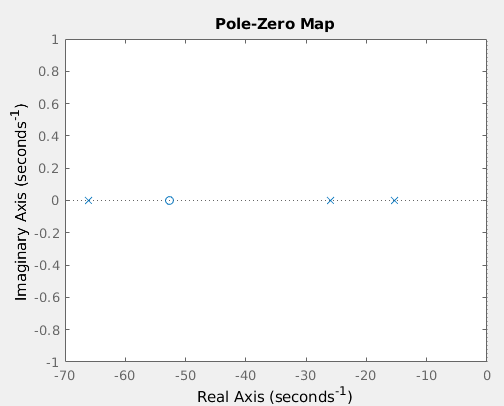
\includegraphics[width=0.7\linewidth]{FTlazoc_pzmap}}
	\caption{Gráfico de Polos y Ceros del Sistema.}
	\label{fig:cp2}
	\end{figure} 
	
Los polos dominantes del sistema son -15.42 y -26.03, debido a que son los más cercanos al eje imaginario, y la distancia entre ellos es relativamente pequeña comparada con la distancia al otro polo.\\
Respuesta de la función de transferencia de lazo cerrado a una señal de entrada escalón de 10V:

  \begin{figure}[H] % Example image
	\center{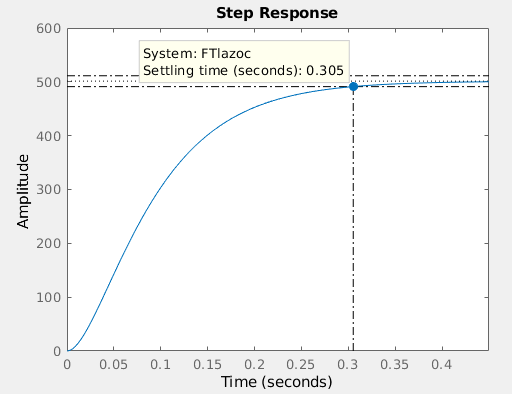
\includegraphics[width=0.7\linewidth]{FTlazoc_step}}
	\caption{Respuesta de la función de transferencia de lazo cerrado a una señal de entrada escalón de 10V.}
	\label{fig:resp_esc2}
	\end{figure} 

De la grafica se puede observar el error de estado estable del 50\% ya que el sistema fue estimulado con un entrada de 10V, para la cual correspondería una salida de 1000lm. El tiempo de asentamiento es de alrededor de 300ms, que es compatible con el tipo de aplicación. La respuesta no presenta sobrepasamiento.\\
Respuesta de la función de transferencia a lazo cerrado ante una señal de entrada tipo rampa:

  \begin{figure}[H] % Example image
	\center{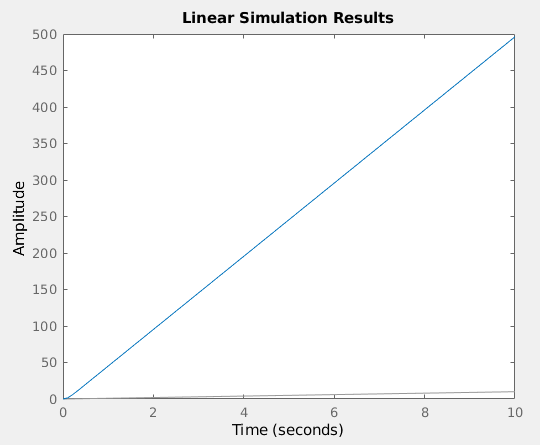
\includegraphics[width=0.7\linewidth]{FTlazoc_ramp}}
	\caption{Respuesta de la función de transferencia a lazo cerrado ante una señal de entrada tipo rampa.}
	\label{fig:resp_rampa1}
	\end{figure} 
Como puede observarse la respuesta del sistema ante una entrada tipo rampa presenta un error que tiende al infinito correspondiente a lo que deberíamos esperar para un sistema de tipo 0.

\section{Lugar de Raíces}

Graficar el lugar de raices es una herramienta muy utilizada en los analisis de los sistemas de control. Con esta se puede determinar si el sistema es estable para cualquier ganancia, o para determinar los valores de ganancia para los que el sistema se mantiene estable:

  \begin{figure}[H] % Example image
	\center{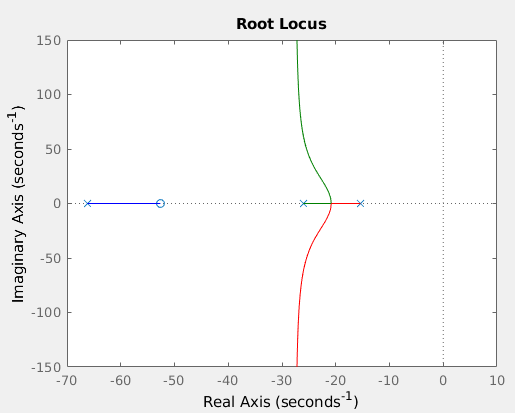
\includegraphics[width=0.7\linewidth]{FTlazoc_rlocus}}
	\caption{Gráfico del Lugar de Raíces.}
	\label{fig:FTlazoc_rlocus}
	\end{figure} 


 \begin{figure}[H] % Example image
	\center{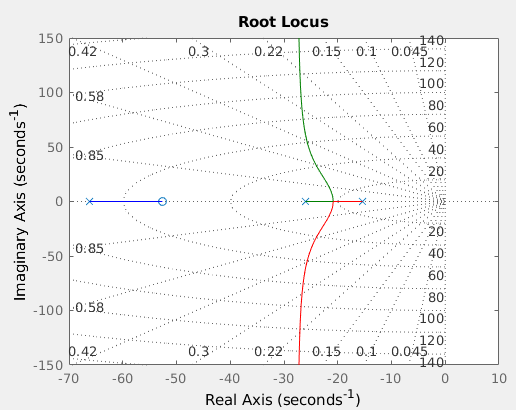
\includegraphics[width=0.7\linewidth]{FTlazoc_sgrid}}
	\caption{Gráfico del Lugar de Raíces con lineas de zeta constante.}
	\label{fig:FTlazoc_sgrid}
\end{figure}


\begin{figure}[H] % Example image
	\center{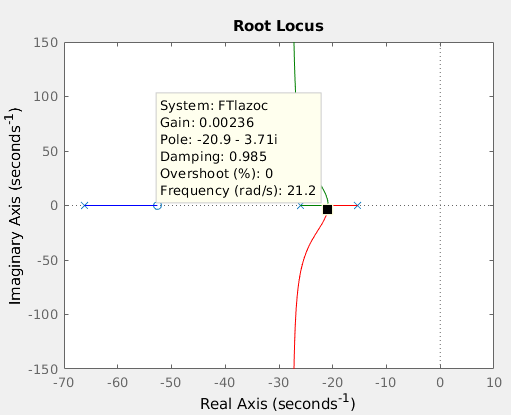
\includegraphics[width=0.7\linewidth]{FTlazoc_rlocus_overshoot0}}
	\caption{Gráfico del Lugar de Raíces con marcador sobre el último valor de la raíz sobrepaso cero.}
	\label{fig:FTlazoc_rlocus_zeta1}
\end{figure} 

En el grafico se ve que al tener todo el lugar de raíces en la parte real negativa del grafico el sistema sera estable para cualquier valor de ganancia mayor a cero, esto es para k>0.
El sistema será sobreamortiguado para valores de 0 a 0.0023.A partir del valor k=0.0024 en adelante existirá sobrepasamiento por lo que la respuesta sera subamortiguada. Entonces existe amortiguado crítico para k=0.0024.\\


 
A continuación se muestran tres gráficos para los distintos valores de k, para mostrar las distintas formas en las que reacciona el sistema.

Para k=0,0001. Sistema sobreamortiguado.

  \begin{figure}[H] % Example image
	\center{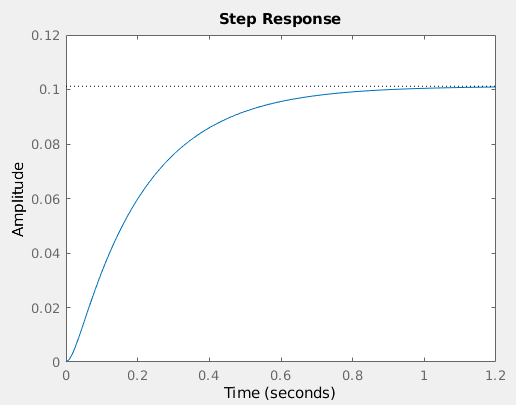
\includegraphics[width=0.7\linewidth]{FTlazoc_k00001}}
	\caption{Respuesta de la función de transferencia a lazo cerrado ante una señal de entrada tipo escalón para un k=0,0001.}
	\label{fig:FTlazoc_k00001}
	\end{figure} 

Del grafico se observa que no hay sobrepaso, debido al sobreamortiguamiento, pero el valor en estado estable es menor a 0.1lm y es demasiado bajo. El error de estado estable aumento muchísimo, esto es debido a que la ganancia agregada es muy baja.

Para k=10. Sistema subamortiguado.

  \begin{figure}[H] % Example image
	\center{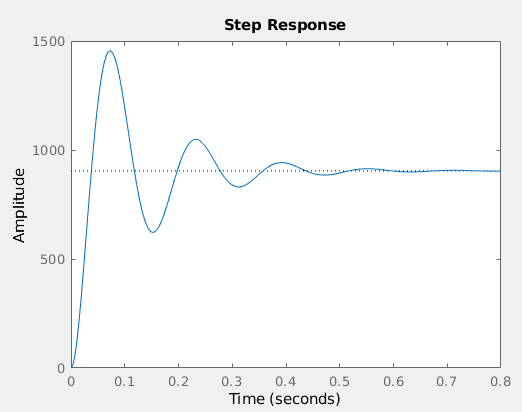
\includegraphics[width=0.7\linewidth]{FTlazoc_k10}}
	\caption{Respuesta de la función de transferencia a lazo cerrado ante una señal de entrada tipo escalón para un k=10.}
	\label{fig:FTlazoc_k10}
	\end{figure} 

Aquí, al contrario que en el caso sobreamortiguado, se puede ver que hay un sobrepaso muy elevado. Y debido a las oscilaciones que se observan se puede concluir que al sistema le cuesta llegar al valor de régimen permanente. Por otro lado el valor de régimen es próximo al deseado, es decir que se tiene un bajo error de estado estable.\\
Para k=0,0023. Sistema Con amortiguamiento critico.\\

  \begin{figure}[H] % Example image
	\center{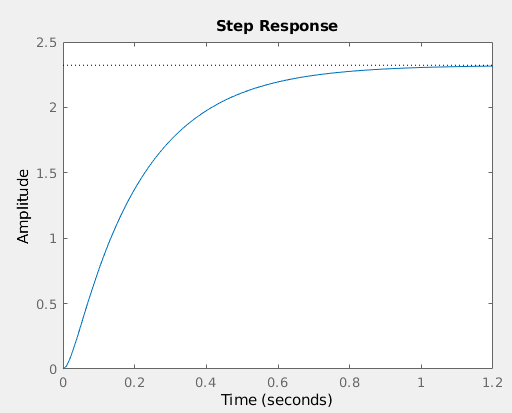
\includegraphics[width=0.7\linewidth]{FTlazoc_kcritico}}
	\caption{Respuesta de la función de transferencia a lazo cerrado ante una señal de entrada tipo escalón para un k=0,0023.}
	\label{fig:FTlazoc_kcritico}
	\end{figure} 
	
Se tiene una salida sin sobrepaso, y un tiempo de asentamiento bajo, pero el error es muy grande, como en el caso de sobreamortiguamiento.
	
\section{Compensación}

\textsc{Requerimientos:}\\
-Error de estado estable: 5\%\\
-Tiempo de establecimiento: 0.3 segundos\\
-Sobrepaso máximo: 5\%\\

Si bien la especificación indica un error de estado estable de 5\%, como máximo es conveniente tener el menor error posible, y como tenemos un sistema de tipo 0 se agregará un polo en el origen. Esto hará que el sistema pase a ser de tipo 1.
El integrador que se agrego al sistema será:$$\frac{1}{s}$$
Y al estimular el sistema con una entrada escalón de 10V se tiene un error de estado estable de 0\%.\\
	
  \begin{figure}[H] % Example image
	\center{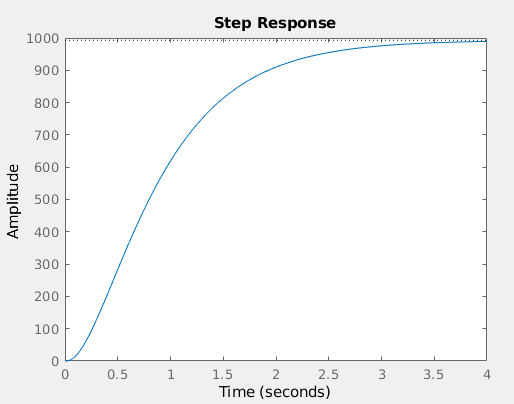
\includegraphics[width=0.7\linewidth]{FTlazoc_poloenorig_step}}
	\caption{Respuesta de sistema con el integrador ante una señal de entrada escalón de 10V.}
	\label{fig:FTlazoc_poloenorig_step}
	\end{figure} 

Como ya se dijo el error es 0\%, pero el tiempo de asentamiento se elevo considerablemente, ahora se tiene un tiempo aproximado de 4 segundos.

En el gráfico siguiente se muestra el nuevo lugar de raíces una vez agregado el integrador, y ademas se agrega una imagen ampliada en la región cercana al eje imaginario:\\

  \begin{figure}[H] % Example image
	\center{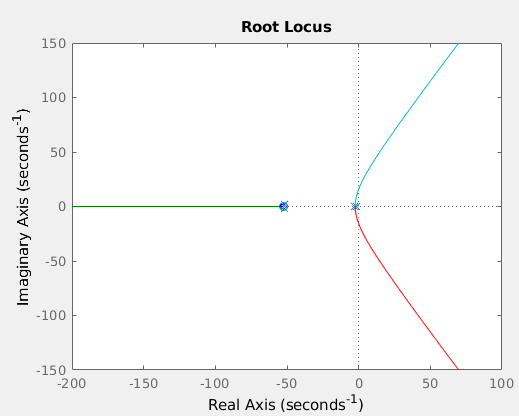
\includegraphics[width=0.7\linewidth]{FTlazoc_poloenorig_rlocus}}
	\caption{Grafico de lugar de Raíces para el sistema con integrador.}
	\label{fig:FTlazoc_poloenorig_rlocus}
	\end{figure} 

	  \begin{figure}[H] % Example image
	\center{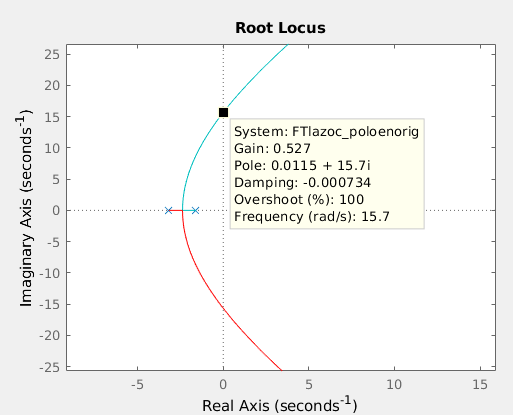
\includegraphics[width=0.7\linewidth]{FTlazoc_poloenorig_rlocus_zoom}}
	\caption{Acercamiento al origen sobre el grafico de lugar de Raíces para el sistema con integrador.}
	\label{fig:FTlazoc_poloenorig_rlocus_zoom}
	\end{figure} 

Lo primero que se puede observar es que las líneas del lugar de raíces se desplazaron considerablemente hacia la parte positiva del eje real por lo que para valores de $k>0.527$ el sistema es inestable.
En esta ultima figura se ve que el sistema sera estable para $0<k<0.527$. Sera sobreamortiguado para $k<0.00134$, subamortiguado para $0.00134<k<0.527$. Y sera críticamente amortiguado para $k = 0.00134$.\\
Para controlar este tiempo de establecimiento y llevarlo al valor especificado en los requerimientos debemos diseñar un compensador. Teniendo en cuenta el requerimiento de sobrepaso máximo se puede calcular el valor de $\zeta$:\\
$$0,05=e^{\frac{-\pi*\zeta}{\sqrt{1-\zeta^{2}}}}$$
Se obtiene un $\zeta$ de 0.707. Y teniendo en cuenta el requerimiento de tiempo de asentamiento calculamos el valor para la frecuencia Wn:
$$T_s=\frac{4}{\zeta*W_n} $$
$$W_n=\frac{4}{\zeta*T_s}=\frac{4}{0,707*0.3}$$
$$W_n=18.86$$
Con estos valores obtenidos se calculara el punto de diseño:
$$S = - \zeta*W_n + i*W_n*\sqrt{1-\zeta^2}$$
$$S = - 0,707*18.86 + i*18.86*\sqrt{1-0,707^2}$$
$$S = -13.33+13.33i$$
Como este punto de diseño no pertenece al lugar de raíces del sistema, y no puede ser alcanzado con una ganancia. Se procederá a diseñar un compensador que modifique el lugar de raíces para que contenga el punto de diseño.\\
Se tendrá en cuenta para el análisis la Función de Transferencia de lazo abierto contemplando el polo en el origen:
$$FT_{LA+int_{(ZPK)}}=\frac{13409}{s(s + 52.63)(s + 50)(s + 5)}$$
Los polos de la función de transferencia de lazo abierto, incluyendo el integrador son:\\
\begin{center}
$P_0=0$\\
$P_1=-5$\\
$P_2=-50$\\
$P_3=-52.63$\\
\end{center}

Los ángulos aportados por cada polo respecto al punto de diseño son:\\
\begin{center}
$$\angle_{P_0}=180\degree-tg^{-1}(\frac{13.33}{13.33-0})=135\degree$$
$$\angle_{P_1}=180\degree-tg^{-1}(\frac{13.33}{13.33-0})=132.8\degree$$
$$\angle_{P_2}=tg^{-1}(\frac{13.33}{13.33-0})=19.8\degree$$
$$\angle_{P_3}=tg^{-1}(\frac{13.33}{13.33-0})=18.8\degree$$
\end{center}

%[AGREGAR LAS FORMULAS GENERICAS COMO EN EL OTRO TRABAJO, el que paso santiago]

Con estos ángulos se puede calcular el angulo del compensador teniendo en cuenta la condición de fase o ángulo:
$$\sum_{i}\angle_{C_i}=\sum_{n}\angle_{P_n} - \sum_{m}\angle_{Z_m}=180\degree$$
$$135\degree+132,8\degree+19.8\degree+18.8\degree = 180\degree$$
$$306.4\degree \ne 180\degree$$
Entonces será necesario agregar un polo y un cero en adelanto de manera que quedará la sumatoria de fases:
$$135\degree+132,8\degree+19.8\degree+18.8\degree+ \angle_{P_c} - \angle_{Z_c}= 180\degree$$
pero si coloco el cero del compensador sobre el polo en -5 entonces tengo que $\angle_{Z_c}=135 \degree $
$$135\degree+132,8\degree+19.8\degree+18.8\degree+ \angle_{P_c} - 132.8\degree= 180\degree$$
$$\angle_{P_c} = 180\degree - 135\degree-19.8\degree-18.8\degree$$
$$\angle_{P_c} = 6.4\degree$$

El compensador que debemos utilizar es un compensador en adelanto que nos permita disminuir el tiempo de establecimiento al valor de requerimiento.
Conociendo el ángulo que debe aportar el polo del compensador es posible calcular el valor de la raiz sobre el eje real negativo mediante trigonometría:
$$P_c=\frac{13.33}{tg^{-1}6.4\degree}+13.33$$
$$P_c=\frac{13.33}{0.11}+13.33$$
$$P_c=134.51$$

Entonces quedan definidos el cero del compensador en -5 y el polo en -134,51. Dado que el cero está más próximo al eje imaginario se cumple que es un compensador en adelanto.

Para calcular la ganancia del compensador se utilizará la condición de módulo:
$$K_{TOTAL}=\frac{\prod_n P_n}{\prod_m Z_m}$$
$$K_{TOTAL}=\frac{H_0\times H_1\times H_2\times H_3+H_4}{H_{Z_c}}$$
Pero $H_1=H_{Z_c}$ entonces:
$$K_{TOTAL}=H_0\times H_2\times H_3\times H_4$$
Los valores de los módulos se obtienen aplicando Pitágoras:
$$K_{TOTAL}=12.85\times 39.02\times 41.5\times 121.91$$
$$K_{TOTAL}=3721266$$
Teniendo en cuenta que:
$$K_{TOTAL}=K_{FTLA_int}\times K_{COMP}$$
$$K_{COMP}=\frac{3721266}{13409}$$
$$K_{COMP}=277.5$$


%[ACA IRIA EL GRAFICO DEL COMPENSADOR]

\begin{table}[h!]
\centering
\caption{Cero, Polo y Ganancia del Compensador calculado.}
\begin{tabular}{c}
\hline
\hline 
$\displaystyle Cero = -5$\tabularnewline
$\displaystyle Polo = -134.51$\tabularnewline
$\displaystyle Kc=277.5$\tabularnewline
\hline
\hline
\end{tabular}
\end{table}

La función de transferencia resultante para el compensador PID es:
$$PID=277.5\times\frac{s+5}{s(s+134.51)}$$
Agregando el compensador al diagrama de bloques el sistema resulta:\\

  \begin{figure}[H] % Example image
	\center{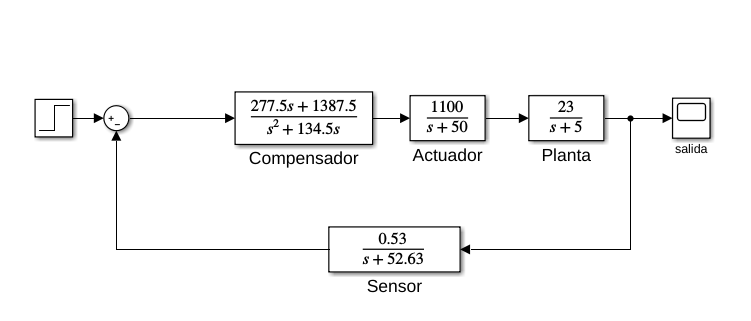
\includegraphics[width=0.7\linewidth]{slink_comp}}
	\caption{Diagrama de bloques con el Compensador PID.}
	\label{fig:slink_comp}
	\end{figure} 
	
Las funciones de transferencia del sistema agregando el PID resultan:
$$FT_{LA_{PID}}=\frac{13409s+67045}{s^5+242.1s^4+1.762\text{e-}4s^3+4.361\text{e-}5s^2+1.77\text{e-}6s}$$
$$FT_{LA_{PID_{(ZPK)}}}=13409\times\frac{s+5}{s(s+134.5)(s+52.63)(s+50)(s+5)}$$
y a lazo cerrado
%$$FT_{LC_{PID}}=\frac{259s^2+531s+272}{0,001386s^5+0,1559s^4+1,794s^3+5,939s^2+6,89s+2,72}$$
%$$FT_{LC_{PID_{(ZPK)}}}=186807\times\frac{(s+1,05)(s+1)}{(s+100)(s+7,93)(s+0,9-0,26i)(s+0,9+0,26i)s}$$
EL lugar de raíces del sistema habiendo agregado el PID resulta:

  \begin{figure}[H] % Example image
	\center{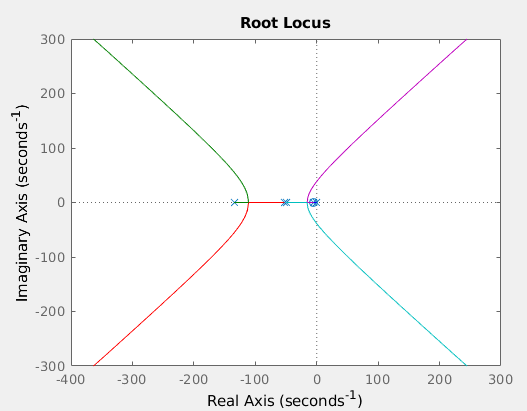
\includegraphics[width=0.7\linewidth]{FTlazoa_comp_rlocus}}
	\caption{Gráfico del Lugar de Raíces para el sistema con Compensador.}
	\label{fig:FTlazoa_comp_rlocus}
	\end{figure} 
	
	  \begin{figure}[H] % Example image
	\center{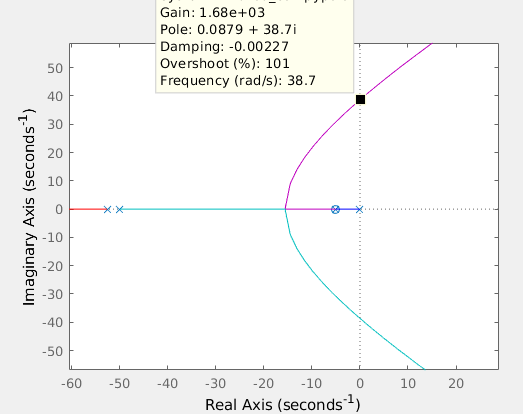
\includegraphics[width=0.7\linewidth]{FTlazoa_comp_rlocus_kinest}}
	\caption{Gráfico del Lugar de Raíces para el sistema con Compensador, con acercamiento en la zona cercana al eje imaginario.}
	\label{fig:FTlazoa_comp_rlocus_kinest}
	\end{figure} 

\begin{figure}[H] % Example image
	\center{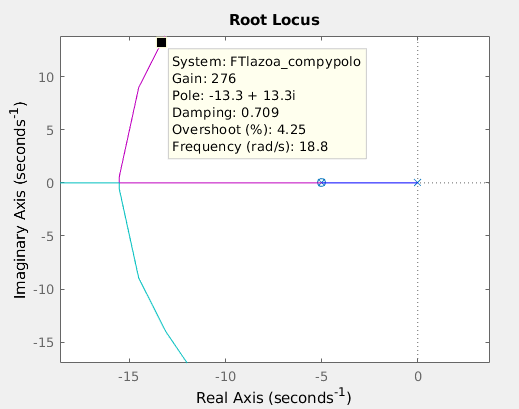
\includegraphics[width=0.7\linewidth]{FTlazoa_comp_rlocus_zoom_kcomp}}
	\caption{Gráfico del Lugar de Raíces para el sistema con Compensador, con marcador sobre el punto del polo de diseño.}
	\label{fig:FTlazoa_comp_rlocus_zoom_kcomp}
\end{figure} 

Se puede ver claramente que el sistema es inestable para un $k>1.67\text{e}3$. También se valida el valor obtenido para la ganancia del compensador utilizando un marcador sobre el punto de diseño y obteniendo el valor de la ganancia por interpolación.\\
A continuación se muestra la salida del sistema compensado para una entrada escalón de 10V:	
	
	  \begin{figure}[H] % Example image
	\center{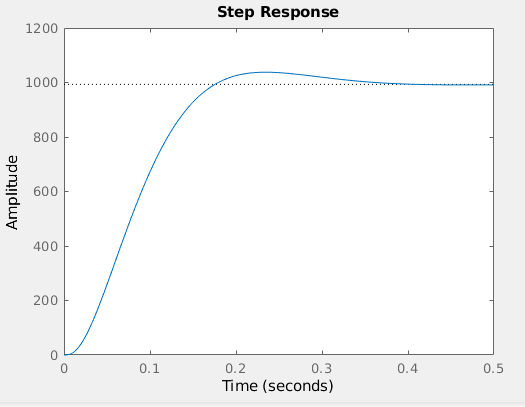
\includegraphics[width=0.7\linewidth]{FTlazoc_comp_step}}
	\caption{Respuesta del sistema compensado ante una señal de entrada escalón de 10V.}
	\label{fig:FTlazoc_comp_step}
	\end{figure} 

 \begin{figure}[H] % Example image
	\center{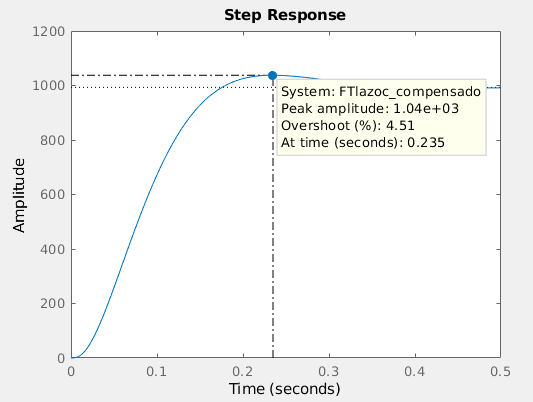
\includegraphics[width=0.7\linewidth]{FTlazoc_comp_step+sobrepaso}}
	\caption{Lectura del sobrepaso para la respuesta del sistema compensado ante una señal de entrada escalón de 10V.}
	\label{fig:FTlazoc_comp_step+sobrepaso}
\end{figure} 

 \begin{figure}[H] % Example image
	\center{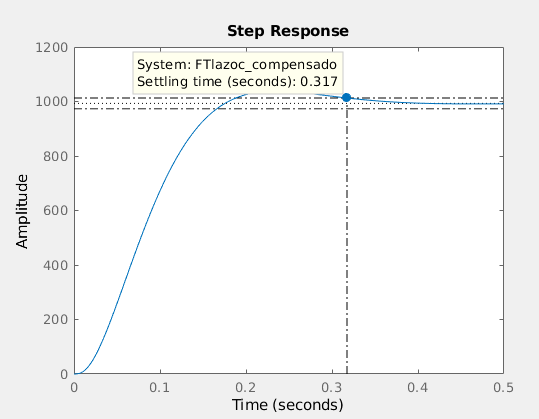
\includegraphics[width=0.7\linewidth]{FTlazoc_comp_step+ts}}
	\caption{Lectura del tiempo de establecimiento para la respuesta del sistema compensado ante una señal de entrada escalón de 10V.}
	\label{fig:FTlazoc_comp_step+ts}
\end{figure} 

 \begin{figure}[H] % Example image
	\center{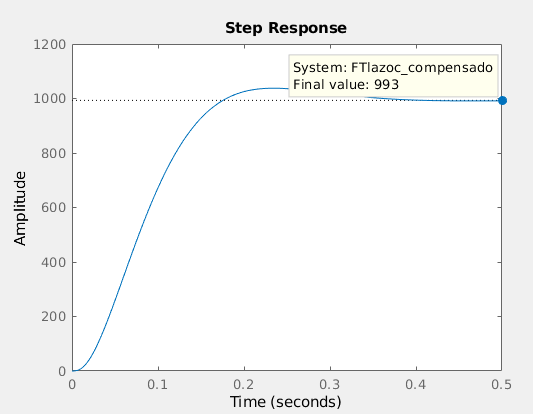
\includegraphics[width=0.7\linewidth]{FTlazoc_comp_step+vf}}
	\caption{Lectura del valor de régimen para la respuesta del sistema compensado ante una señal de entrada escalón de 10V.}
	\label{fig:FTlazoc_comp_step+vf}
\end{figure} 

Se puede ver que se cumplen los requerimientos pretendidos para el sistema. El sobrepaso es menor al 5\%. El error de estado estable es despreciable ya que la salida para un escalón de 10V de entrada es de 1000lm (es la deseada). Y el requerimiento respecto al tiempo de establecimiento de 300 milisegundos se cumple con apenas una variación de 17ms totalmente despreciable para el tipo de aplicación.


\section{Respuesta del Sistema ante distintas Perturbaciones}

En esta sección se producirán distintas perturbaciones en la salida del sistema, para observar como responde el sistema ante las mismas. Como entrada del sistema, para todos los casos, se tendrá una señal escalón de 8V. Para esta entrada se espera tener una salida de 800lm.

 \begin{figure}[H] % Example image
	\center{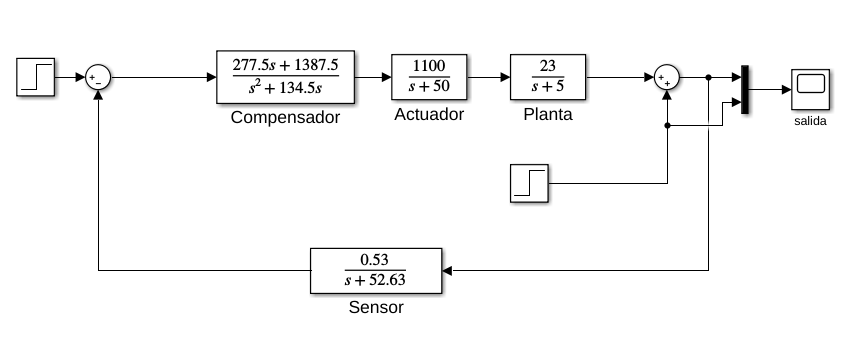
\includegraphics[width=0.7\linewidth]{slink_comp_pert}}
	\caption{Modelo de simulink empleado para evaluar el efecto de las perturbaciones.}
	\label{fig:slink_comp_pert}
\end{figure} 

El siguiere gráfico muestra la salida, al introducir una señal escalón de 100lm a la salida del sistema a los 5 segundos, luego de que se haya llegado al estado estable:\\

	  \begin{figure}[H] % Example image
	\center{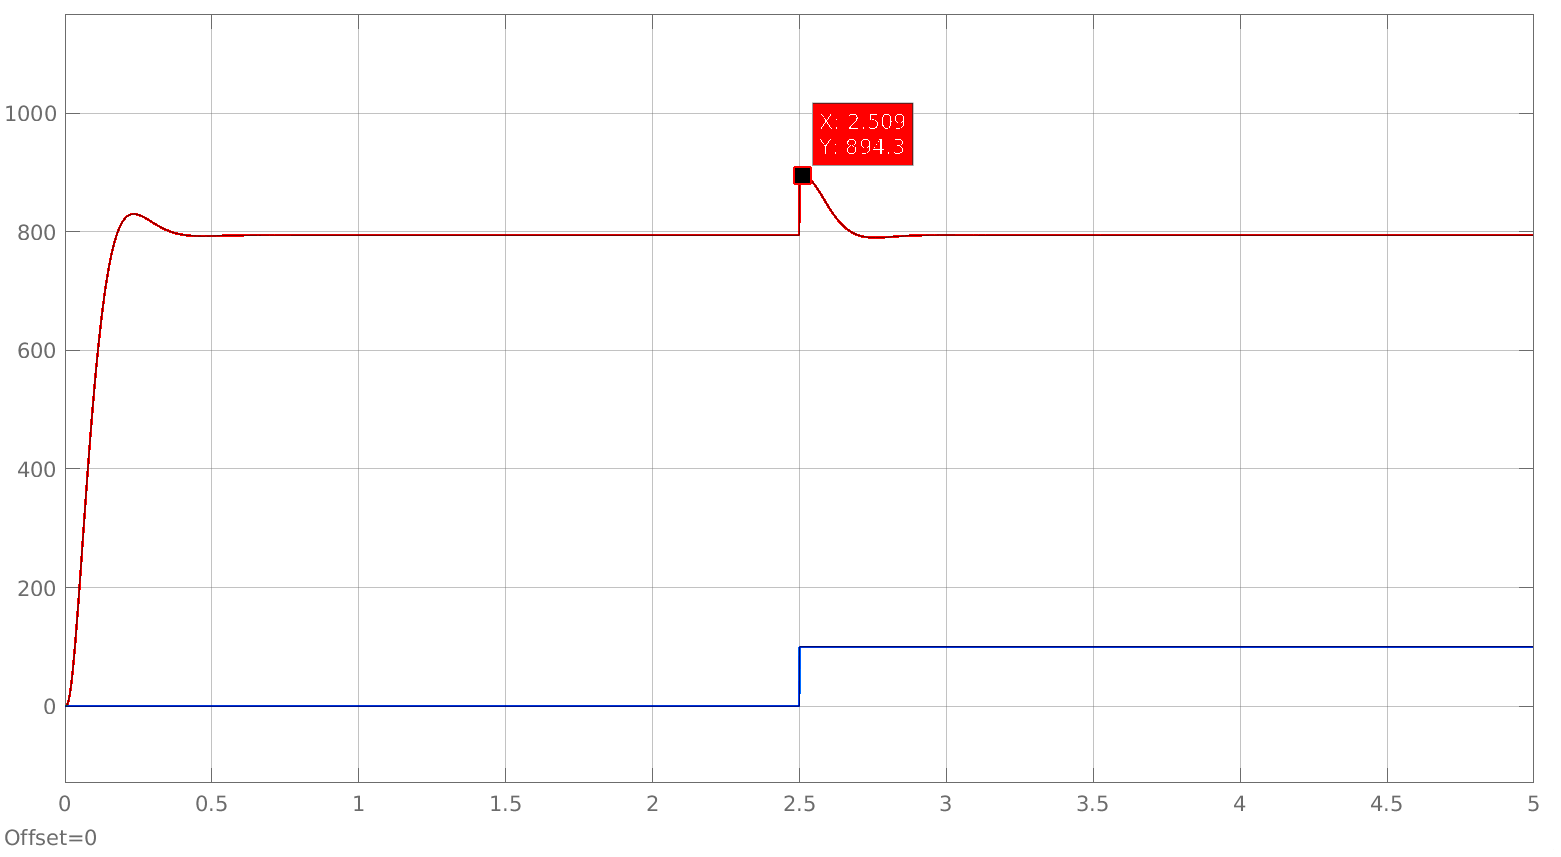
\includegraphics[width=0.7\linewidth]{FTlazoc_comp_step+pert_escalon}}
	\caption{Respuesta del sistema compensado ante una señal de ruido tipo escalón de 100lm inyectada en la salida una vez alcanzado el régimen.}
	\label{fig:FTlazoc_comp_step+pert_escalon}
	\end{figure} 

Se aprecia como el sistema se ve afectado, debido a que la entrada es repentina, pero luego de unos segundos logra superar esa perturbación, acomodando la salida al valor deseado de 800lm.\\
La siguiente perturbación corresponde a una rampa, con una pendiente de 20 lúmenes por segundo, introducida a los 2.5 segundos de comenzada la simulación. El sistema alcanzo su estado estable:\\

	  \begin{figure}[H] % Example image
	\center{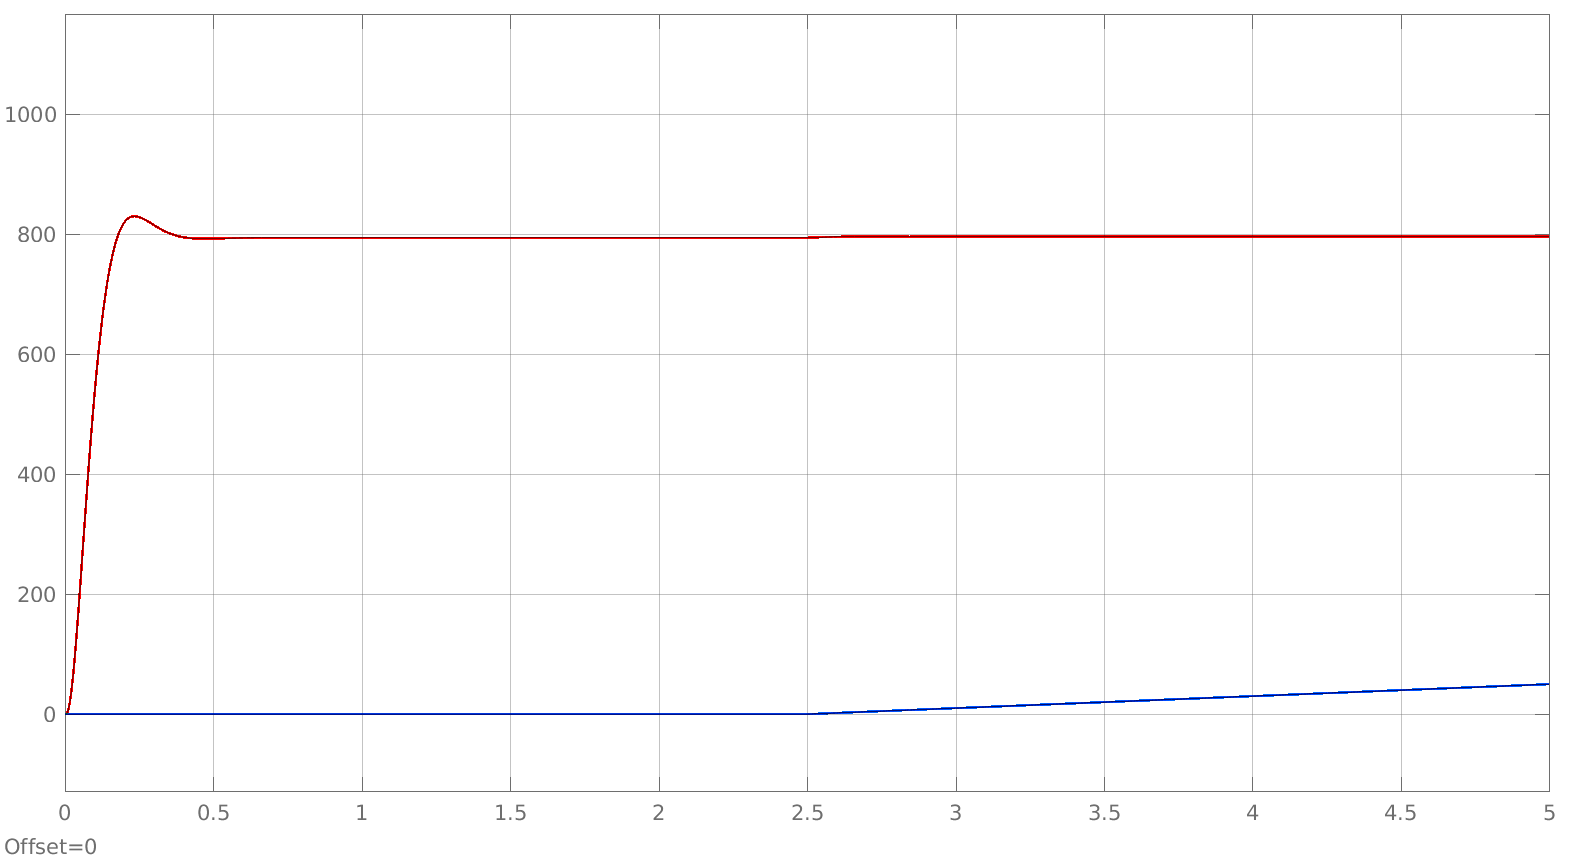
\includegraphics[width=0.7\linewidth]{FTlazoc_comp_step+pert_ramp}}
	\caption{Respuesta del sistema compensado ante una señal de ruido tipo rampa con pendiente de 20lm por segundo inyectada en la salida una vez alcanzado el régimen.}
	\label{fig:FTlazoc_comp_step+pert_ramp}
	\end{figure} 

El sistema prácticamente no se ve afectado por la introducción de esa perturbación ambiental y logra mantener el valor deseado de 800lm.\\
Por último se perturbará el sistema con una señal senoidal, con un frecuencia de 1Hz y 3Hz, y una amplitud de 100lm. Esta perturbación esta desde el inicio de la simulación:\\

	  \begin{figure}[H] % Example image
	\center{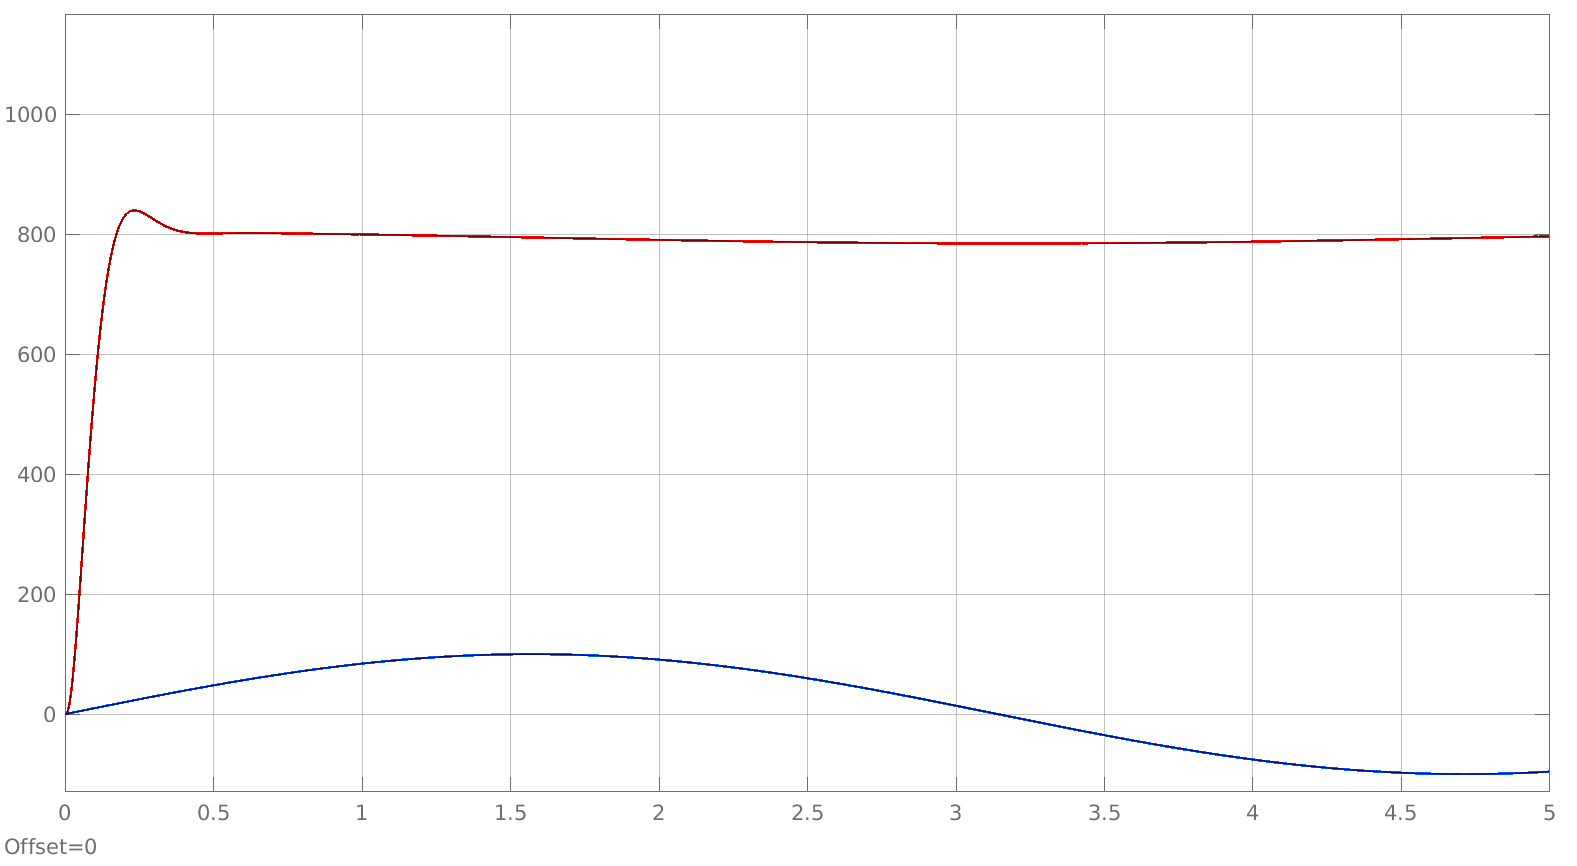
\includegraphics[width=0.7\linewidth]{FTlazoc_comp_step+pert_sin1hz}}
	\caption{Respuesta del sistema compensado ante una señal de ruido tipo senoidal de 1Hz inyectada en la salida.}
	\label{fig:FTlazoc_comp_step+pert_sin1hz}
	\end{figure}

 \begin{figure}[H] % Example image
	\center{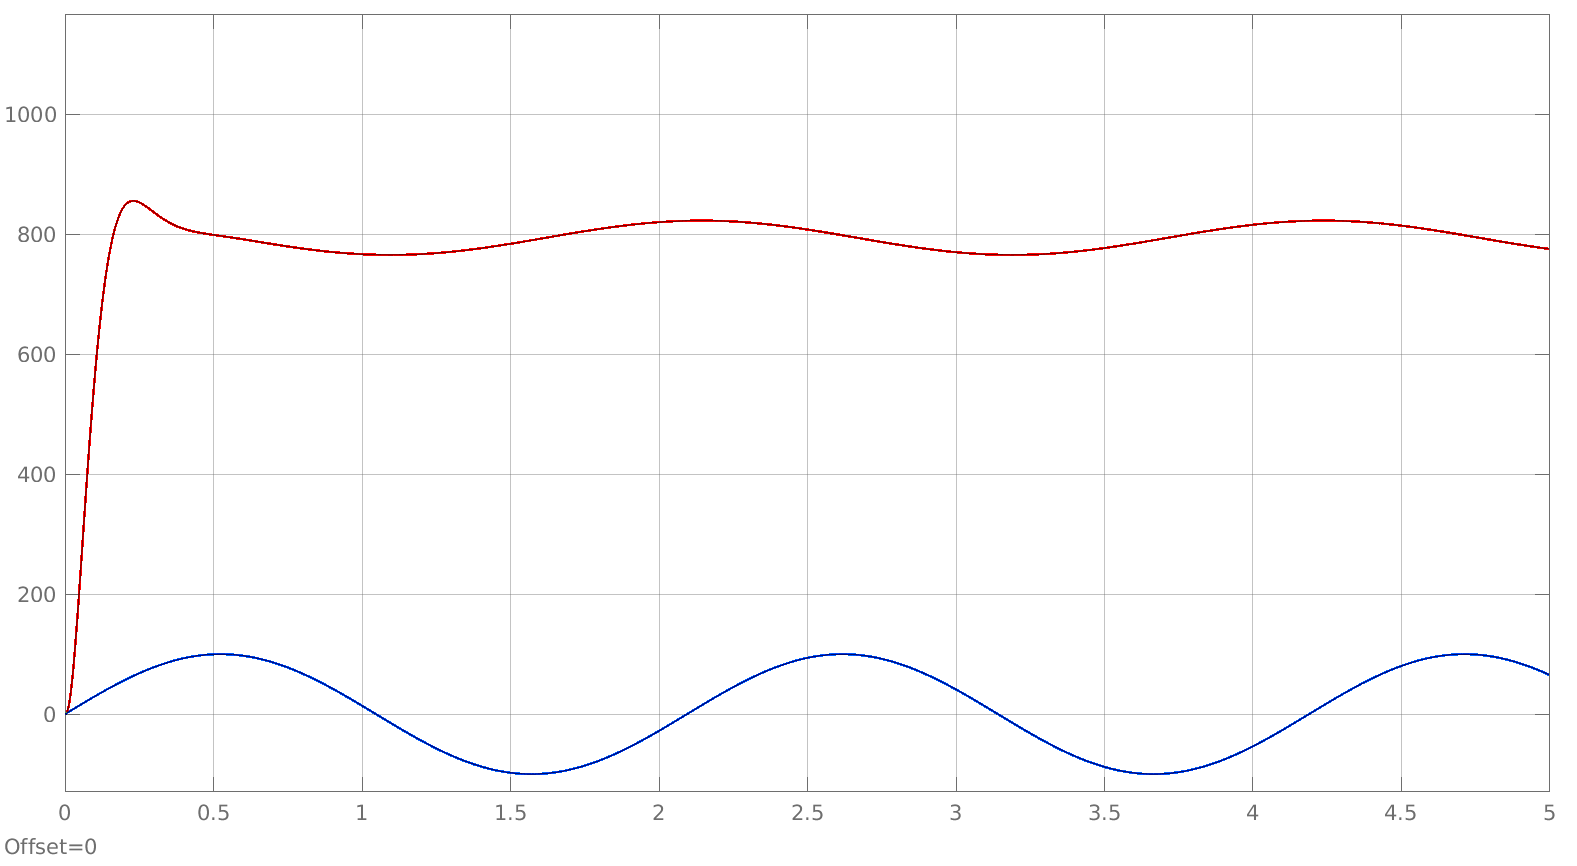
\includegraphics[width=0.7\linewidth]{FTlazoc_comp_step+pert_sin3hz}}
	\caption{Respuesta del sistema compensado ante una señal de ruido tipo senoidal de 3Hz inyectada en la salida.}
	\label{fig:FTlazoc_comp_step+pert_sin3hz}
\end{figure}
	
Se puede ver como el sistema atenúa la amplitud de la perturbación, oscilando entre 770lm y 830lm, alrededor del valor deseado de 800lm.\\
Si se aumenta la frecuencia de oscilación el sistema ya no consigue dicha atenuación y se podrían evidenciar errores mayores al 5\% que se admitió como requerimiento de diseño. Pero para los propósitos de este trabajo esa frecuencia es elevada ya que es muy improbable que se produzcan variaciones tan rápidas en la luminosidad de un ambiente.
Ademas se ha simulado el sistema con la misma señal con una frecuencia mas baja, de 0.01Hz. El sistema ha sido capaz de controlarla y mantenerse en el valor deseado de 800lm, teniendo un error de estado estable admisible por la consigna.\\

\section{Respuesta en Frecuencia}
\sloppy
La respuesta en régimen permanente de un sistema a señales sinusoidales en un rango de frecuencias es lo que se conoce como la respuesta en frecuencia del sistema.\\
El interés de tratar entradas sinusoidales está en que la respuesta del sistema a estas señales contiene información sobre la respuesta a señales más generales. De hecho, toda señal periódica puede descomponerse en una sumatoria de senos y cosenos, por el Teorema de Fourier. Conociendo la respuesta del sistema a las componentes sinusoidales de la señal de entrada, puede reconstruirse por Fourier la señal de salida.\\
A continuación se muestra el Diagrama de Bode del Sistema en Lazo Abierto sin y con el compensador:\\

	\begin{figure}[H] % Example image
	\center{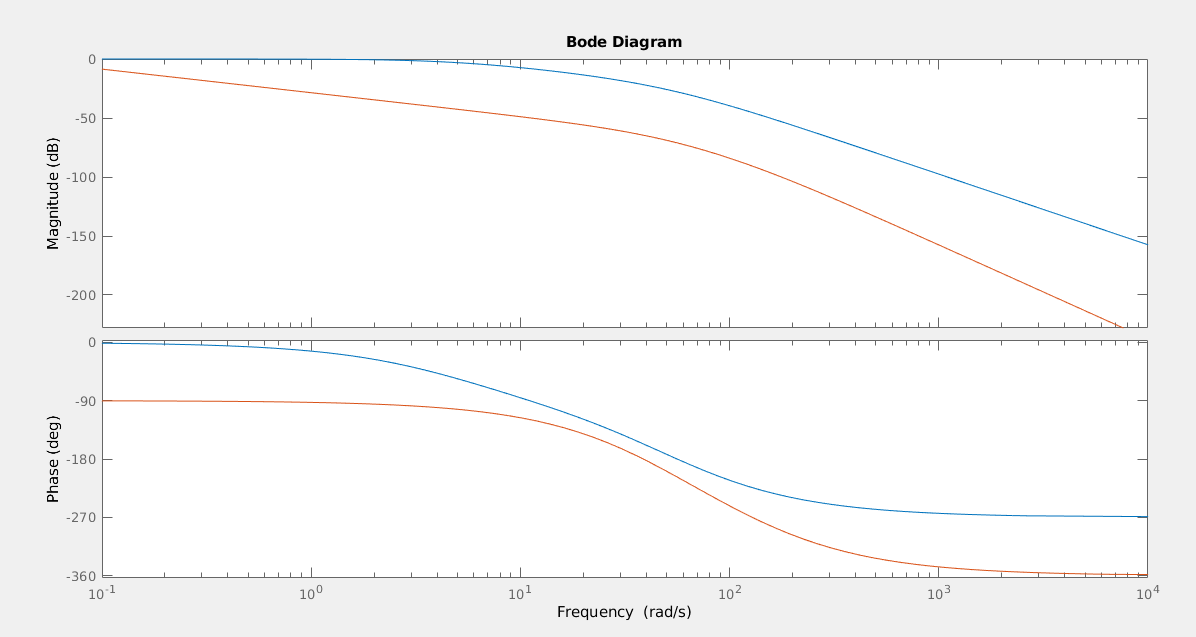
\includegraphics[width=\linewidth]{bode_la+la_comp}}
	\caption{Diagrama Bode de ambas funciones, en azul a Lazo Abierto sin Compensador
	y en verde con Compensador.}
	\label{fig:bode_la+la_comp}
	\end{figure}
	
Hay dos parámetros que miden la estabilidad relativa de un sistema de control:
\begin{itemize}
\item Margen de Fase.
\item Margen de Ganancia.
\end{itemize}

\textsc{Margen de Fase}

El margen de fase es la cantidad de atraso de fase adicional en la frecuencia de cruce de ganancia requerida para llevar el sistema al borde de la inestabilidad.\\
Sea $\omega_{FCGan}$ la frecuencia de cruce de ganancia es la frecuencia tal que hace que $|FT(j\omega_{FCGan})|=1\rightarrow 0dB$. Si $\phi(j\omega_{FCGan})$ es el ángulo del sistema de lazo abierto, entonces el margen de fase se define como:

$$M_{frec}=180\degree+\phi(j\omega_{FCGan})$$

\textsc{Margen de Ganancia}

El margen de ganancia es el recíproco de la magnitud $|G(j\omega)|$ en la frecuencia a la cual el ángulo de fase es -180° . Si $\omega_{FCFase}$ es esta frecuencia, entonces se define como:

$$M_{gan}=\frac{1}{|FT(j\omega_{FCFase})|}$$
En deciBeles:\\
$$M_{gan_{dB}}=20\times\log M_{gan}=-20\times\log|FT(j\omega_{FCFase})|$$

Para un sistema estable de fase mínima, el margen de ganancia indica cuánto puede incrementarse la ganancia antes de que el sistema se vuelva inestable. Para un sistema inestable, el margen de ganancia indica cuánto debe disminuir la ganancia para que el sistema se vuelva estable.

	\begin{figure}[H] % Example image
	\center{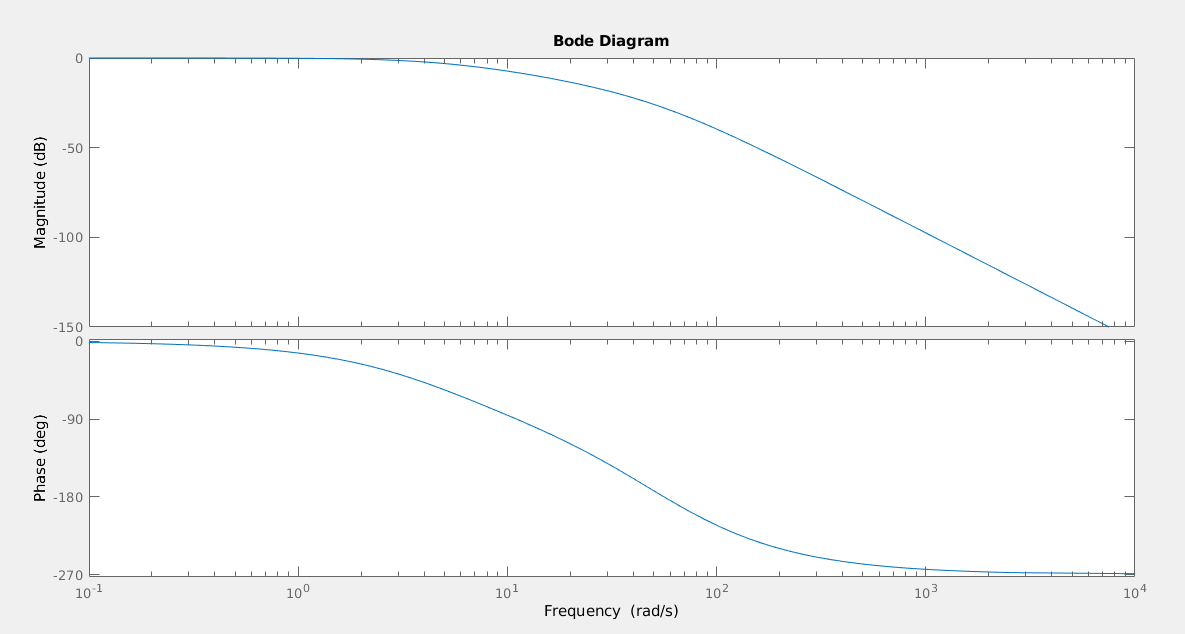
\includegraphics[width=\linewidth]{bode_la}}
	\caption{Diagrama de Márgenes de la función de transferencia a lazo abierto sin compensador.}
	\label{fig:bode_la}
	\end{figure}
	
	\begin{figure}[H] % Example image
	\center{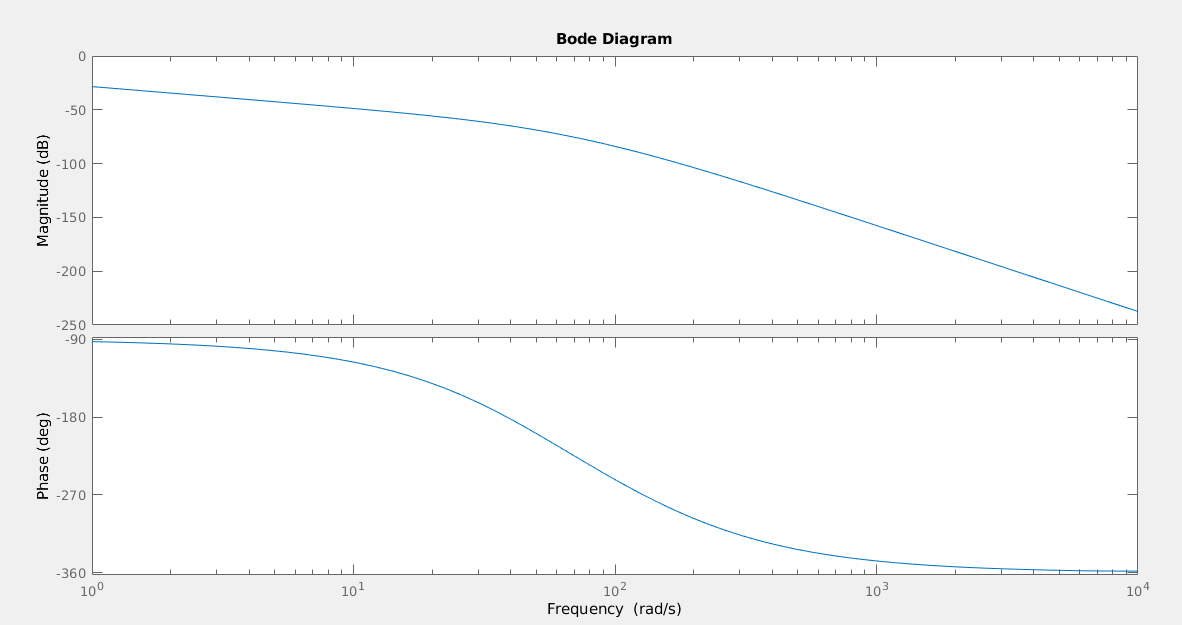
\includegraphics[width=\linewidth]{bode_la_comp}}
	\caption{Diagrama de Márgenes de la función de transferencia a lazo abierto con compensador.}
	\label{fig:bode_la_comp}
	\end{figure}
	
	\begin{figure}[H] % Example image
	\center{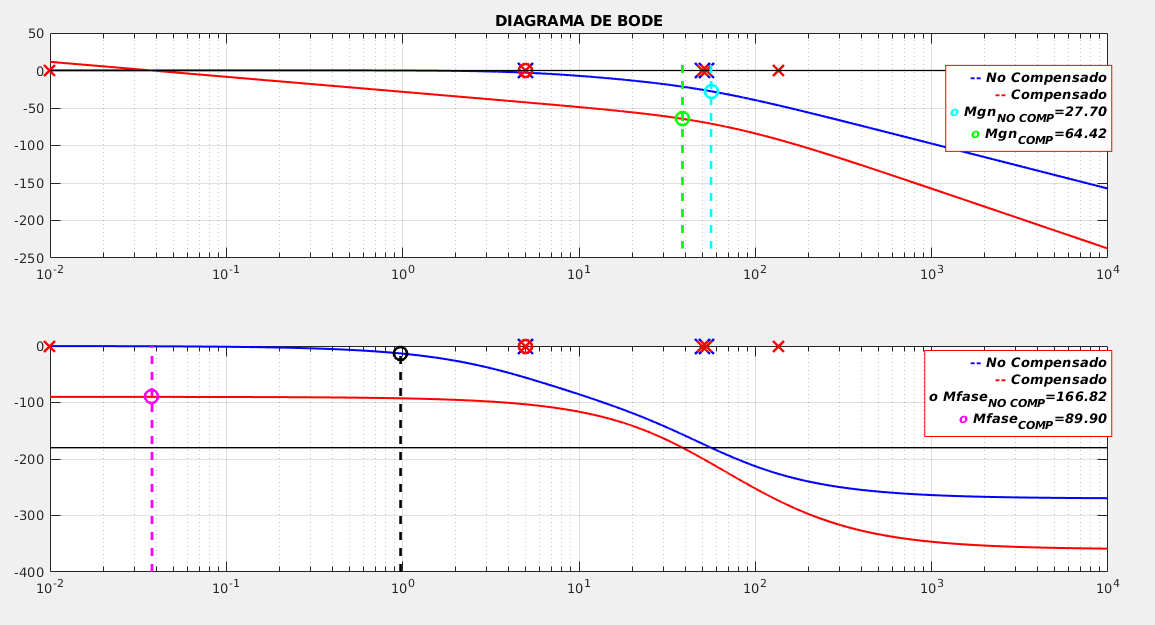
\includegraphics[width=\linewidth]{bode_margenFymargenG}}
	\caption{Diagrama de Bode con los márgenes, ceros y polos.}
	\label{fig:bode_margenFymargenG}
	\end{figure}

\begin{table}[h!]
\centering
\caption{Valores obtenidos del Análisis en Frecuencia.}
\begin{tabular}{|c|c|}
\hline
$LA_{NO COMP}$ & $LA_{COMPENSADO}$\tabularnewline
\hline
\hline 
$M_{gan}=27.70[dB]$ & $M_{gan}=64.42[dB]$\tabularnewline
\hline 
$M_{frec}=-166.82\degree $ & $M_{frec}=-89.90\degree $\tabularnewline
\hline 
$\omega_{FCGan}=0[\frac{rad}{seg}]$ & $\omega_{FCGan}=0[\frac{rad}{seg}]$\tabularnewline
\hline
\end{tabular}
\end{table}

Como puede observarse en los gráficos y más fácilmente en Cuadro 5  los valores para los márgenes tanto de ganancia como el de fase acusan estabilidad para la versión sin y con compensador de la función de transferencia de Lazo Abierto del Sistema.
En cuanto a la frecuencia de cruce de ganancia $\omega_{FCGan}$ se observa un desplazamiento positivo de 0,616 rad/seg por eso la disminución en el margen. 

\section{Código Matlab}
%\begin{lstlisting}[language=Octave,caption=Codigo Fuente usado para el trabajo.]
%\end{lstlisting}
\lstinputlisting{control2021.m}%[caption=Codigo fuente principal Matlab.]
\vspace*{5\baselineskip}
\lstinputlisting{dibujar_BodeFINAL.m}%[caption=Codigo fuente funcion dibujar_Bode.]
\end{document}
